\subsection{Nachbearbeitung der Vorhersagen}
\label{sec:Nachbearbeitung}
Mit dem trainierten Modell können nun Vorhersagen erzeugt werden.
In \autoref{lst:Prediction} ist dieser Prozess anhand eines zufälligen Beispiels aus den Validierungsdaten gezeigt.

\begin{code}
\begin{minted}[
    linenos,
    numbersep=10pt,
    gobble=0,
    frame=lines,
    framesep=2mm]{python}
def predict_random_example(model, val_dataset):
    example = val_dataset[np.random.choice(range(len(val_dataset)), size=1)[0]]
    x = np.expand_dims(example[0:-1, ...], axis=0)
    y_true = np.squeeze(example[-1, ...])
    y_pred = np.squeeze(model.predict(x))

    return y_true, y_pred
\end{minted}
\captionof{listing}{Erzeugung einer Vorhersage anhand der Validierungsdaten}
\label{lst:Prediction}
\end{code}

Dafür wird in Zeile 1 zunächst eine zufällige Sequenz von 17 Frames aus den Validierungsdaten ausgewählt.
In Zeile 2 und 3 wird die Sequenz in die Eingabe- und Zieldaten unterteilt, die dann jeweils in die richtige Form gebracht werden.
Die eigentliche Vorhersage findet dann in Zeile 5 statt, wo sie durch \emph{model.predict(x)} ausgeführt wird.
Die Arrays \emph{y\_true} und \emph{y\_pred} enthalten nun die Wahren und die vorhergesagten Ergebnisse und haben die Form $(50,~50)$.
In \autoref{fig:PredExProb} sind zwei Beispiele für Vorhersagen grafisch dargestellt.

\begin{figure}[h]
    \centering
    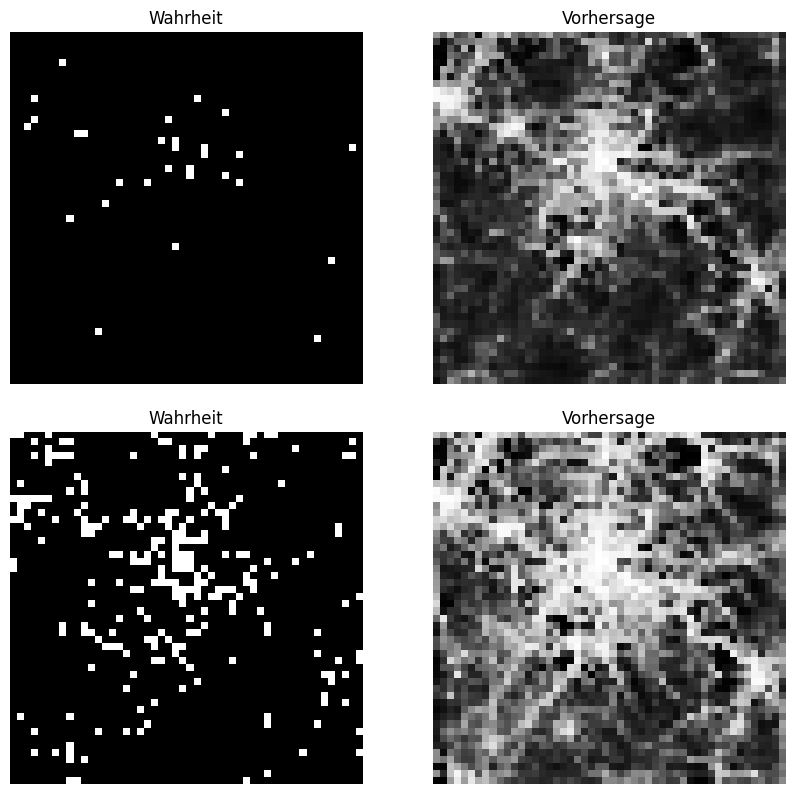
\includegraphics[width=1.0\textwidth,height=12cm,keepaspectratio=true]{content/images/PredExProb.png}
    \caption{Beispiele für Vorhersagen des trainierten Modells (rechts) im Vergleich zur Realität (links)}
    \label{fig:PredExProb}
\end{figure}

Links im Bild sieht man die realen Standorte der mobilen Radarkontrollen.
Rechts hingegen ist die Ausgabe des \acrshortpl{nn} dargestellt.
Je dunkler die Pixel, desto geringer ist der Zahlenwert und umgekehrt.
Zunächst kann man leicht erkennen, dass nicht alle Pixel schwarz sind, sondern dass ein weiter Bereich an Zahlenwerten abgedeckt wird.
Das spricht dafür, dass die gewichtete Verlustfunktion ihren Zweck erfüllt.
Als nächstes ist erkennbar, dass das Modell scheinbar teilweise das Straßennetz erlernt hat.
In den Vorhersagen sind große Straßen als Linien und große Städte als Cluster deutlich erkennbar.
Dies ist durchaus nachvollziehbar, da die Radarkontrollendichte hier besonders hoch ist.
Dadurch stellt sich jedoch die Frage, ob die Vorhersage des Modells überhaupt maßgeblich von der Eingabe abhängig ist.
Dafür spricht jedenfalls der Unterschied zwischen dem oberen und unteren Beispiel.
Im oberen Beispiel sind in der Realität deutlich weniger Radarkontrollen vorhanden als im unteren Beispiel.
Das könnte beispielsweise dadurch zustande kommen, dass das obere Beispiel von einem Samstag oder Sonntag stammt.
In der bereits diskutierten \autoref{fig:AnzahlNachWochentag} ist schließlich deutlich zu erkennen, dass es am Wochenende deutlich weniger Radarkontrollen gibt als unter der Woche.
Auch die Vorhersage spiegelt diesen Sachverhalt wieder.
Während die Vorhersage im oberen Beispiel viele dunkle Pixel enthält, ist die Vorhersage im unteren Beispiel insgesamt deutlich heller, das Modell geht also insgesamt von einer höheren Wahrscheinlichkeit für mobile Radarkontrollen aus.
% TODO: Vergleich von gleichen Wochentagen? Auf später verweisen?

